
\section{Results}

The model was tested in several experiments. First, the generic dynamics of 
model is inspected. The convergence to equilibrium price is studied with two
simulations and then the model is validated using stylized facts. Then the
market dynamics is examined by injecting shocks to the order book via placement 
preferences of the traders. In all the experiments all the traders are given the 
opportunity make one trading decision per session, meaning that the speak ratio 
is one. There are no dividend nor interest paid for any assets in these experiments.
% TODO: Extend

\subsection{Generic dynamics of the model}
% Price dynamics, stylized facts, order book evolution
The single asset simulation was run three times: for the first run
the starting market price was set to 500, for the second run it
was set to 1 500 and for the third was set to 1 000 which is near the equilibrium price. 
The rationale for this equilibrium price is discussed later.
The first and second simulations were
used to study how the convergence to the equilibrium price occurs
and the third to examine the stylized facts of the price
dynamics after the equilibrium is reached. The simulations were
run with 10 000 zero intelligent traders which is the 
same amount of traders as what \citet{Raberto05} used in their experiments
with somewhat similar settings. As only the converge to equilibrium is 
the point of interest in the first and second simulations, the number of sessions
were chosen to be relatively small, 200 sessions, but to get reliable results for
the third simulation the number of sessions was chosen to be 4 000 in order to 
make sure the statistical significance of the tests performed to validate the 
stylized facts will not be hampered by the number of the observation.

The amount of currency and the amount of stock 
a trader owns in the beginning of all the simulations were set to
10 000 000 units and 10 000 units respectively. Therefore
the ratio of stock to currency is 1 000 which
is the expected equilibrium price as there are
no payouts in either assets. The amount of currency
per trader may seem much but as the tick size is one,
it may be more convenient to think the currency as amounts
of cents or pennies. The standard deviation of
the normal distribution that the traders use to pick the order prices
is set to 20.

%\begin{table}
%    \input{tables/simulation_summary.tex}% table.tex > \mytable
%\end{table}


\subsubsection{Converge to Equilibrium}
% Descriptive analysis:
%   how converge occurs
The evolution of trade prices, quantities and trade values thorough
the trading sessions for the lower and higher starting price simulations 
are shown in the figure ~\ref{fig:basic_trades}. As can be observed,
the near equilibrium market price is achieved before 30 trading
sessions for both runs. The simulation with lower starting price converges
to the equilibrium in almost instantly whereas for the higher starting
price it takes more sessions. Furthermore, the traded quantities are
initially lower for the simulation with higher staring price than 
for the simulation with lower price. As the traded volumes are lower,
the converge occurs slower due to that there are less situations in
which the market price can adapt. In addition to these findings, 
the equilibrium price is a slightly lower than the expected which is 
about 940.
%The reason why the price stays slightly 
%under the equilibrium price and why the price converges quicker with
%lower starting price than with the higher may be caused by the implementation of
%determining the order price and order quantity. If a trader decides
%to allocate less currency on an order than the order price it chose 
%the order gets obviously invalidated but there is no such
%limitation for placing asks. Therefore, there might be a slightly less
%bids than asks in general.

\begin{figure}
    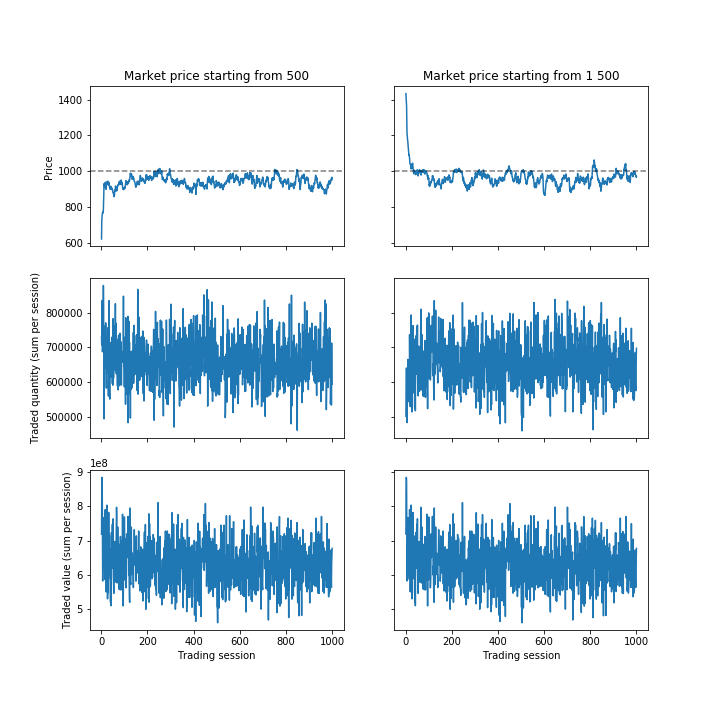
\includegraphics[width=\linewidth]{plots/basic_trades.png}
    \caption{Evolution of price and quantity}
    \label{fig:basic_trades}
\end{figure}

% How the market converged to equilibrium
The market depths, as shown in figure ~\ref{fig:market_depths}, suggest that the
converge to equilibrium is caused by balancing the sides of the market. 
In this figure, the order book is visualized for the first 15 trading sessions
for both of the simulations: with a starting market price of 500 and 1 500. 
The surface describes the evolution of the cumulative bids and cumulative asks 
throughout time and the bottom of the valley formed in the surface is the bid-ask spread. 
The left side from the valley is the cumulative bid book and right is the cumulative ask book. 
The ask side of the market is almost completely missing initially in the run that
starts with lower market price while the opposite is true for the run with higher
initial market price. The ask side of the order book emerges almost instantly 
in the simulation of the lower starting price whereas the converge happens more 
gradually with higher starting price.


\begin{figure}
    \centering
    \begin{subfigure}{.5\textwidth}
      \centering
      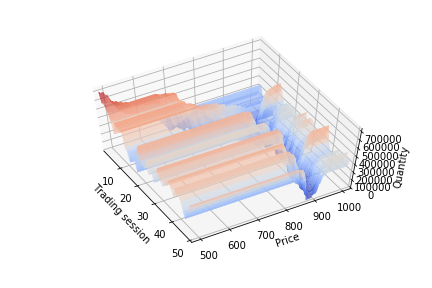
\includegraphics[width=\linewidth]{plots/basic_market_depth_converge_lower.png}
      \caption{Starting price 500}
      \label{fig:market_depth_lower}
    \end{subfigure}%
    \begin{subfigure}{.5\textwidth}
      \centering
      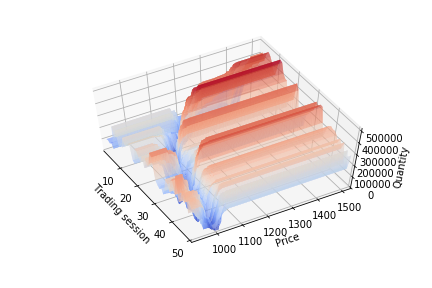
\includegraphics[width=\linewidth]{plots/basic_market_depth_converge_higher.png}
      \caption{Starting price 1 500}
      \label{fig:market_depth_higher}
    \end{subfigure}
    \caption{Converge of the order book to equilibrium}
    \label{fig:market_depths}
\end{figure}

Figure ~\ref{fig:basic_orderbook_evo} provides more top-down view of the orderbook.
This figure shows mostly the same aspects as ~\ref{fig:market_depths} but the sides of the 
order book are not extrapolated to the edges of the plot: the white color represent absence of orders.
The figure suggests that the asking traders in the experiment with lower initial market price
adopt the equilibrium price quicker than the bidding traders in the experiment with higher initial market 
price. One possible explanation for this phenomenon might be the bid-ask asymmetricity
discussed earlier. It is also noteworthy that the downward spikes found in the figure when the equilibrium
is reached is caused by that some traders had consumed most of their currency balances and still decided 
to do a bid order. Because of the budget constrain, these traders had to submit bid orders with prices
they could afford and these prices were substantially lower than the market price and may seem like outliers.

% TODO: Mention that the reason for high price - low price differing convergence to equilibrium is inspected in shocks

\begin{figure}
    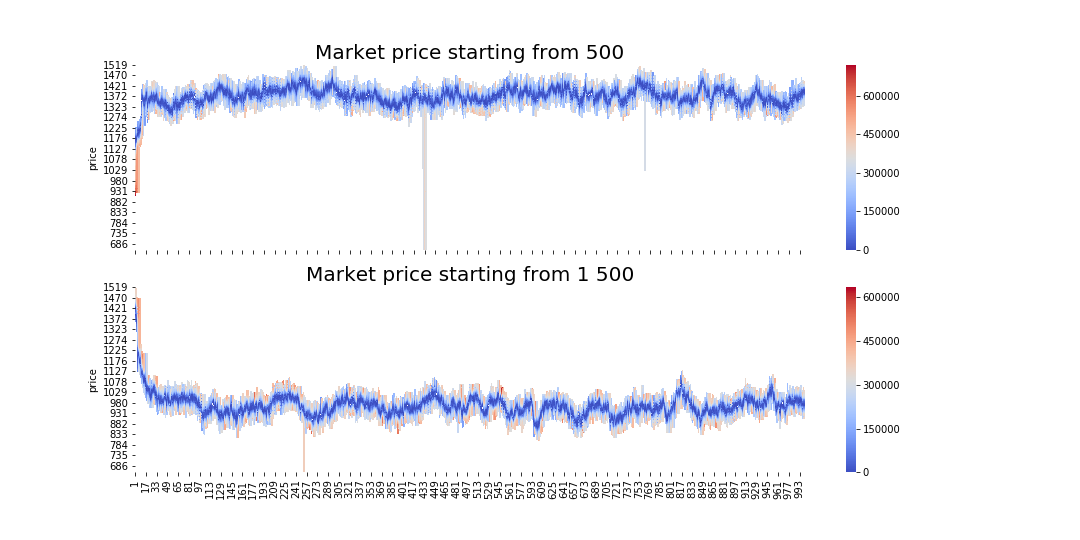
\includegraphics[width=\linewidth]{plots/basic_order_book_evo.png}
    \caption{Order book evolution}
    \label{fig:basic_orderbook_evo}
\end{figure}

When the equilibrium is reached, the order book is rather steep as is illustrated in the figure
~\ref{fig:basic_orderbook_evo}. This figure consists of the last 50 sessions of the extended simulation.
The spread also is also relatively stable most likely due to the number of traders. 

\begin{figure}
    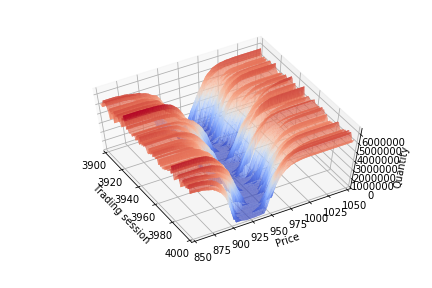
\includegraphics[width=\linewidth]{plots/basic_market_depth_in_equilibrium.png}
    \caption{Order book depth in equilibrium}
    \label{fig:basic_orderbook_evo}
\end{figure}

% TODO: additional finding about explaining the next price

\subsubsection{Stylized Facts}
% stylized facts
% Something about filtering fist 100 out and now inspecting stylized facts
As stated before, the representativeness of the model compared to real markets 
is studied using stylized facts. In order to have representative data set to 
test the stylized facts, the sessions before reaching the price equilibrium are filtered out.
Removing the first 100 sessions was considered suitable for this purpose. 
As already discussed, the longer simulation that starts near equilibrium 
price is used to study the presence of stylized facts in the model. 

% Autocorrelation
% TODO: REWRITE
The autocorrelation function (ACF) and partial autocorrelation function (PACF) for the absolute prices and absolute returns between
the trades are plotted in the figure ~\ref{fig:basic_autocorr}. The absolute returns in this context is the actual price movement of 
the asset and absolute values are simply the actual prices of the asset. As the prices are already in equilibrium, and therefore should be 
stationary, taking third difference from the absolte value, calculating rate of returns, should not be necessary. There is some negative 
autoregressive (AR) process in the absolute returns as the ACF plot shows negative and slowly decaying lags. There are numerous 
significant lags in the AR process as can be observed from the PACF plot. In addition, the prices themselves are 
positively autocorrelated with an AR process as the ACF shows slowly decaying lags. These findings are in line with the experiments conducted by \citet{Raberto05}: 
they also observed some negative autocorrelation in intraday returns and long-lasting autocorrelation in the absolute
values with their simulation. However, it should be noted that this figure shows very short term
autocorrelations and the time between the lags may not be fixed: one lag is simply derived from one
trade. 
% https://www.youtube.com/watch?v=R-oWTWdS1Jg


\begin{figure}
    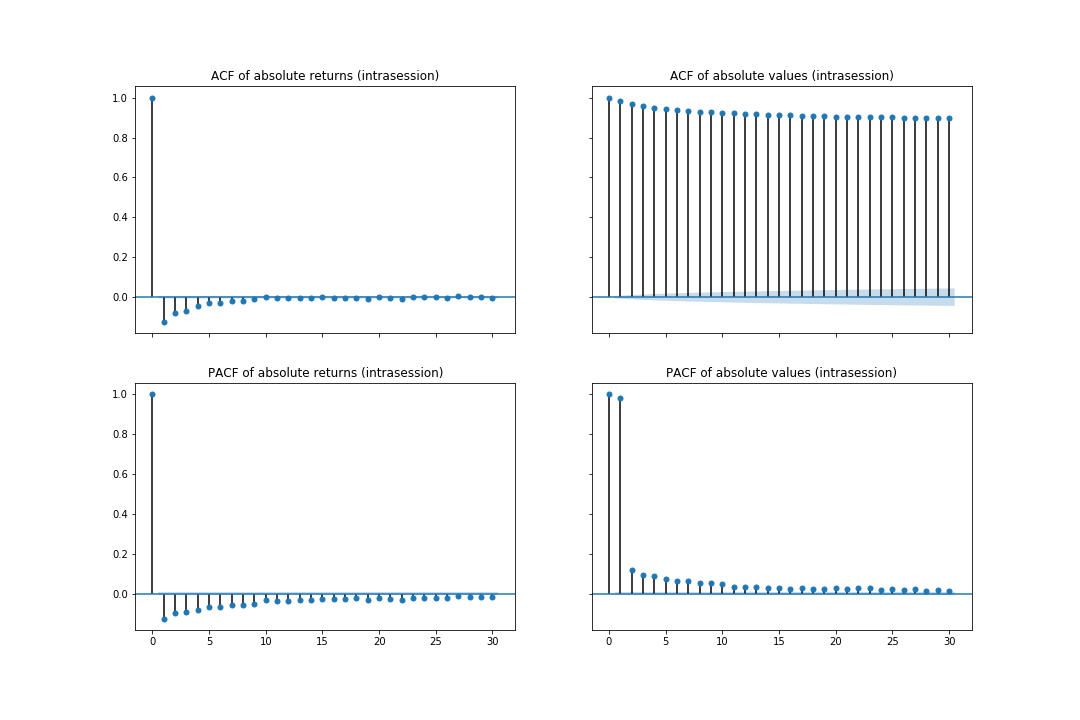
\includegraphics[width=\linewidth]{plots/basic_autocorrelation_intra.png}
    \caption{Autocorrelation of the simulation}
    \label{fig:basic_autocorr}
\end{figure}

Figure ~\ref{fig:basic_autocorr_per_session} suggests that the the autocorrelation is carried over one
session for the absolute returns and four sessions in terms of prices. The prices used in this figure are 
the last trade prices of each session. As can be interpret from the figure, there is an AR(1) process in 
the absolute returns per session and AR(4) for prices on session basis.

\begin{figure}
    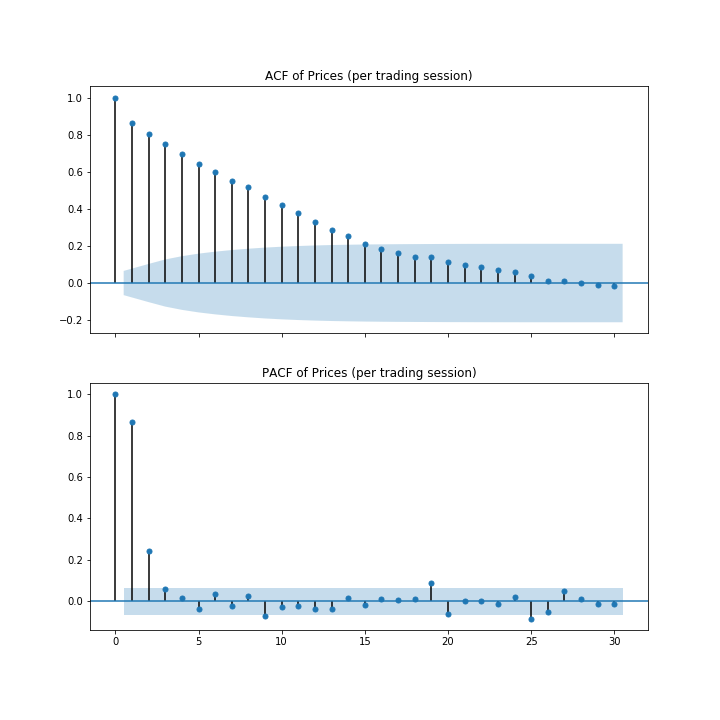
\includegraphics[width=\linewidth]{plots/basic_autocorrelation.png}
    \caption{Autocorrelation of the simulation grouped by session}
    \label{fig:basic_autocorr_per_session}
\end{figure}


% Fat-tailed returns
The distribution of the returns are plotted in ~\ref{fig:basic_return_distr}. As observed in the plot, the fat-tailed returns
clearly exists in the intrasession period but not necessarily per session basis. For intrasession returns, there is a clear spike in the mean of the 
distribution and the tails spread out but these are not visible in the returns between session. In addition, the per session distribution
is not smooth even though the sample consists of 22 million trades. The cause for this may be that the prices are not 
continuous because of the tick size: the minimum possible amount for the price to go up or down is one. Furthermore, prices are
stationary thus the returns are produced by a specific set of prices. Therefore, the returns are also inherently discrete. One option
to mitigate this would be to increase the the amount of currency in order to increase the price and increase the absolute
variation of the prices. Jarque-Bera goodness of fit test suggests that both time periods are not normally distributed,
as the p-values are practically zero in both cases thus the null hypothesis is rejected. The null hypothesis of Jarque-Bera test 
is a joint hypothesis that the distribution has no skewness and no excess kurtosis. However, as discussed, the distributions are not 
convincingly continuous thus it is unclear how robust these results are. The kurtosis of the distribution for intrasession is 5.0 
and -0.5 for session basis and therefore this indicates that the intrasession returns are leptokurtic while the returns between 
sessions are slightly lighter in tails than normal distribution. To summarize, the model does have fatter tails than normal distribution
for intrasession returns but not between sessions. 

% \citet{Raberto05} found fat tails in intra day

\begin{figure}
    \centering
    \begin{subfigure}{.5\textwidth}
        \centering
        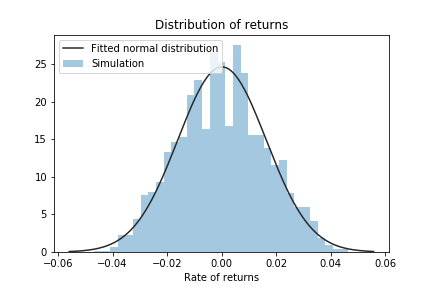
\includegraphics[width=\linewidth]{plots/basic_fat_tails_per_session.png}
        \caption{Between last prices of sessions}
        \label{fig:basic_return_distr_per_session}
    \end{subfigure}%
    \begin{subfigure}{.5\textwidth}
        \centering
        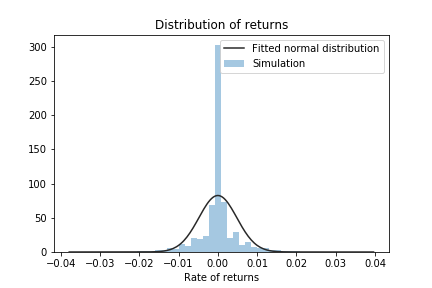
\includegraphics[width=\linewidth]{plots/basic_fat_tails_intrasession.png}
        \caption{Between trades}
        \label{fig:basic_return_distr_intrasession}
    \end{subfigure}
    \caption{Distributions of rate of returns}
    \label{fig:basic_return_distr}
\end{figure}

The spike in the distribution of the intrasession returns may be caused by the structure of the order book. If the order book 
sides are steep, as they are and illustrated in ~\ref{fig:basic_orderbook_evo}, it requires substantially sized 
order to push the opposing side back and have a significant effect on the price. Therefore, the price changes between trades 
are generally rather small until there comes an order that can buy or sell significant chunk of the opposing side and have 
instant impact on the price. In such a case the opposing side may be weakened so much that the price change can be radical. 
Therefore, the reason for the spike in the returns may be that small and medium sized orders may have similar impact on the 
price but big orders may push the side relatively much further as the density of the order quantity in terms of price drops 
when moving further away from the last market price.

% Volatility clusters
The autocorrelation of the volatilities in figure ~\ref{fig:basic_volaclusters}
indicate there are some volatility clusters in short term. The figure was conducted by
dividing the trade prices to a fixed length windows in which the volatilities were calculated per
window basis. As ACF plot is slowly decaying, the autocorrelation follows AR process. The market 
microstructure is able to produce volatility clusters without additional volatility feedback mechanics.
Furthermore, the order book evolution may play a role in the creating the volatility clusters.

\begin{figure}
    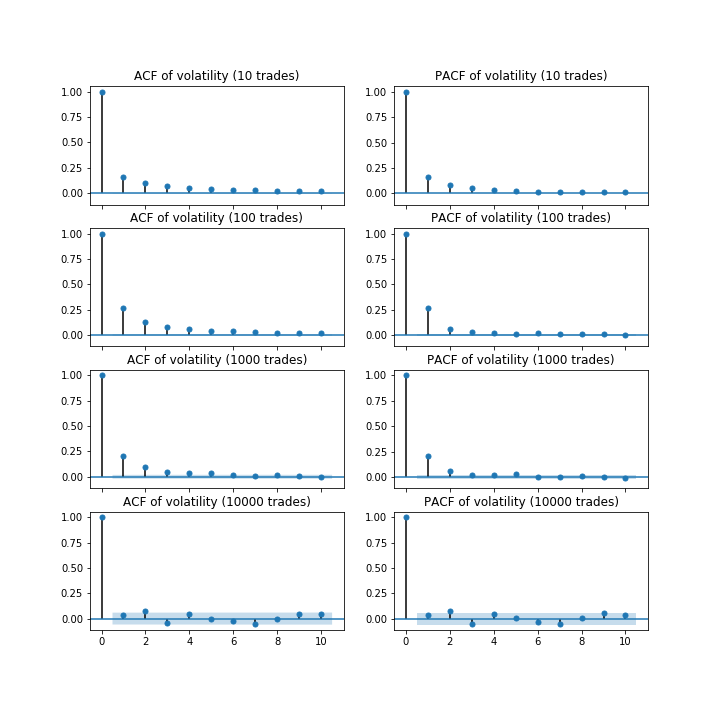
\includegraphics[width=\linewidth]{plots/basic_volaclusters_intra.png}
    \caption{Volatility Clusters}
    \label{fig:basic_volaclusters}
\end{figure}

These findings are somewhat inline with previous literature. \citet{Genoa01}, \citet{Raberto05} and \citet{LIU20082535} 
discussed that the microstructure is the cause for the fat-tailed returns. This is probably also the cause for the
fat-tails of intrasession returns observed in this thesis. However, the autocorrelation is different than what \citet{LIU20082535} 
observed with high call market clearing frequencies. Regardless, the autocorrelations of returns observed in this thesis and in their model
are both short term. Even though a call market has different mechanics than a continuous market, a call market with
very high clearing frequency behaves similarly as a continuous market does. \citet{Genoa01} and \citet{Raberto05} only discussed
about forming volatility clusters in the context of their model which had volatility feedback mechanism thus it is unclear
whether the volatility clusters observed in the model created in this thesis are to be expected.
% TODO: how does the autocorrelation differ from LIU20082535?

\subsection{Shock injection}

To gain better understanding of the order book dynamics of the model the next set of experiments are about injecting shocks 
to the order book. This is done by changing the weights the trading agents use pick the type of an order they will submit. 
The experiment is started in equilibrium and then the probability of picking ask order is increased from 33\% to 43\% 
whereas the probability for bid order is reduced from 33\% to 23\%. The probability for inaction is kept at the 33\%. 
After reaching new equilibrium the weights are set back to 33\% for each option. Then the same experiment is repeated 
but instead of negative shock, positive shock is introduced using weights 43\%, 23\% and 33\% for bid order, ask order 
and inaction respectively. 

As this experiment is more exploratory in nature than the previous experiment the experiment may not need to be computationally
as heavy as the other experiments. Therefore, only 200 sessions are used to let the simulation reach an equilibrium before and during 
the shocks. The number of trading agents are kept at 10 000 to reduce noise in interpreting the results. In addition, both experiments, 
introduction of negative and positive shocks, are conducted in the same simulation run.

The evolution of the order books in both shocks are presented in ~\ref{fig:shocks_orderbook}. Such shocks introduce a new equilibrium
price which is expectedly smaller in negative shock and higher in positive shock. When excess amount of bid orders flow to the market
there is a pressure for the price to increase and vice versa, which is observed here. 
% TODO: Explain when the shocks start and end in the graphs

As observed in the previous experiment, the converge to equilibrium occurs rapidly. Interestingly, the gradual convergence of price
to equilibrium is more prevalent in positive shock than in negative shock. In addition, the order book volumes in both sides of the
market are higher in negative shock than in positive shock, as observed in ~\ref{fig:market_depths_shocks}. Furthermore, the order 
book volumes are higher in negative shock than in the actual equilibrium. The reason for this is most likely that the smaller price 
allows the buyers to bid for higher quantities due to that they can afford more and vice versa. 

\begin{figure}
    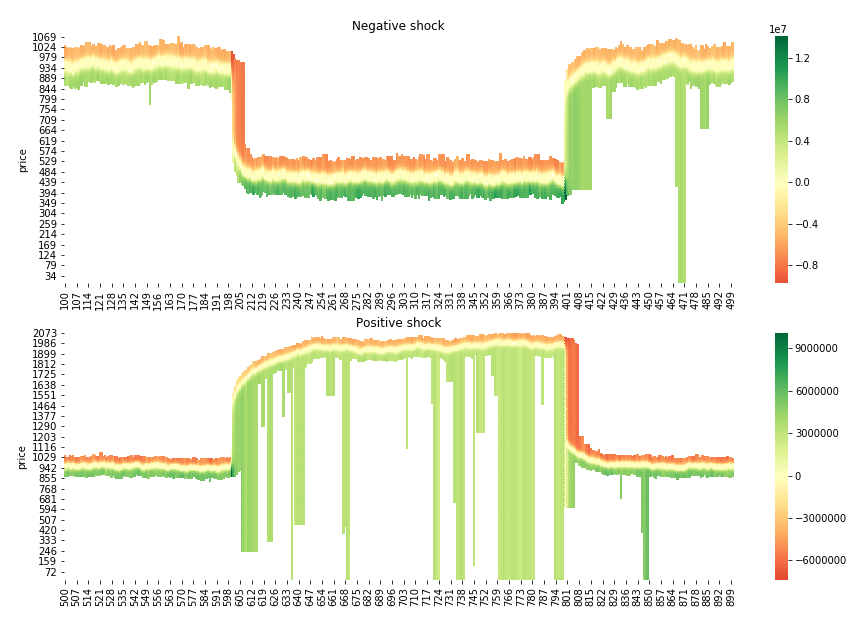
\includegraphics[width=\linewidth]{plots/shocks_order_book_evo.png}
    \caption{Order book evolution in shocks}
    \label{fig:shocks_orderbook}
\end{figure}

The comparable sizes of the order books can be better observed in ~\ref{fig:market_depths_shocks}. Initially in negative shock,
there is a sudden surge of ask orders with sudden decline of bid orders. The existing bid orders are consumed by the ask orders 
until the price reach to levels that the ask orders cannot push further due to the balance between the currency and the asset:
the buyers bid with higher quantities than previously as with the new price they can afford more. Positive shock has similar 
effect: there is a sudden surge of bid orders and the ask side disappears for a moment and then gradually the equilibrium
price is reached as the ask side re-emerges. As demonstrated, the global balance between assets is not the only factor driving the 
market price and the imbalance of the sides of the submitted orders can drive the price also in zero-intelligent markets.

% TODO: There is surge of orders

\begin{figure}
    \centering
    \begin{subfigure}{.5\textwidth}
      \centering
      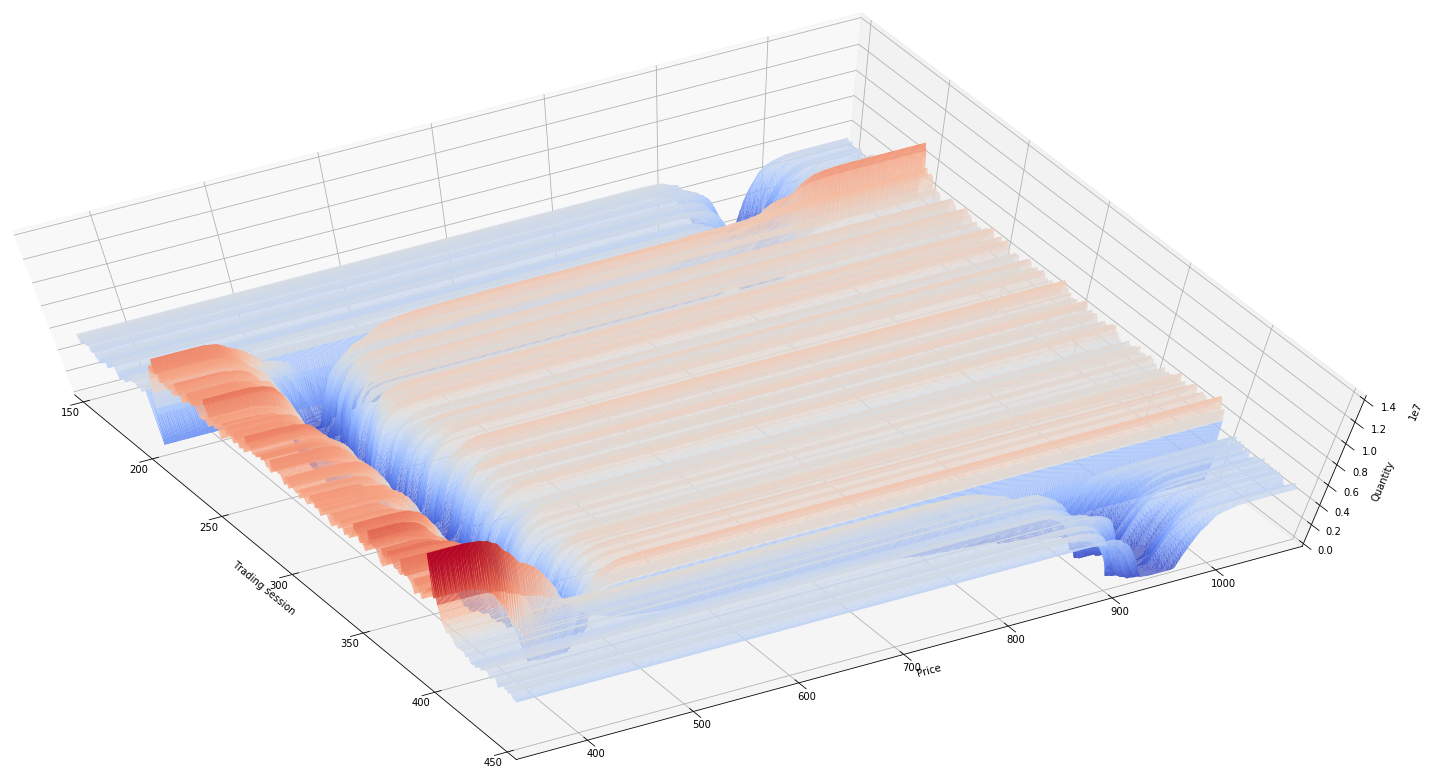
\includegraphics[width=\linewidth]{plots/shocks_neg_market_depth_in_equilibrium.png}
      \caption{Market depth of negative shock}
      \label{fig:market_depth_neg_shock}
    \end{subfigure}%
    \begin{subfigure}{.5\textwidth}
      \centering
      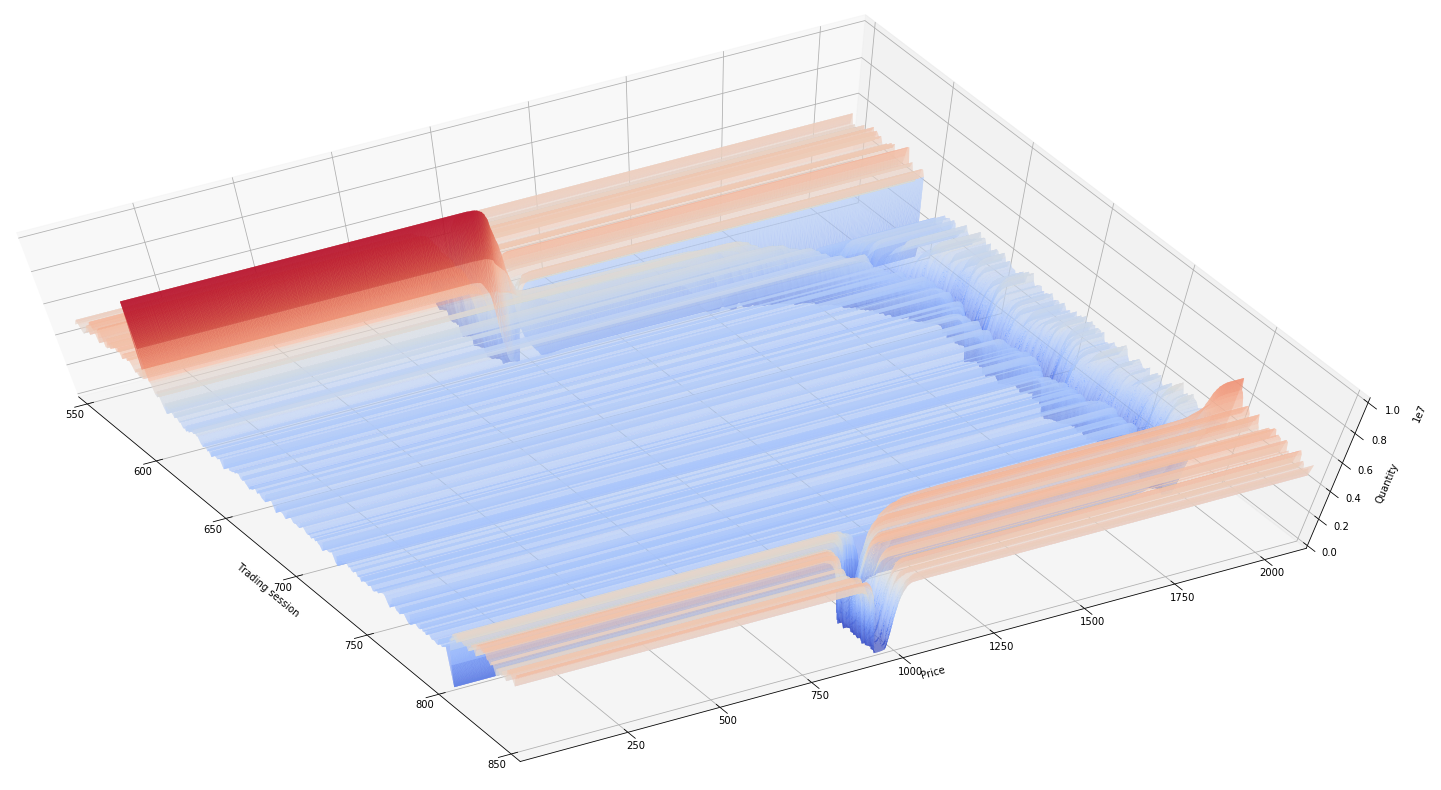
\includegraphics[width=\linewidth]{plots/shocks_pos_market_depth_in_equilibrium.png}
      \caption{Market depth of positive shock}
      \label{fig:market_depth_pos_shock}
    \end{subfigure}
    \caption{Market depths of the shocks}
    \label{fig:market_depths_shocks}
\end{figure}
